The problems described in the previous section lead to the decision of migrating the existing structure to the cloud.

The goal is to create a single cloud-based data warehouse, which can be directly queried by multiple departments both for their needs as well as for performing Business Intelligence analyses.

The communication with the data warehouse is handled by a single could-based integration layer, which is in charge of performing a wide range of operations, from data cleaning to scheduled data retrieval from various sources.

\begin{figure}
    \centering
    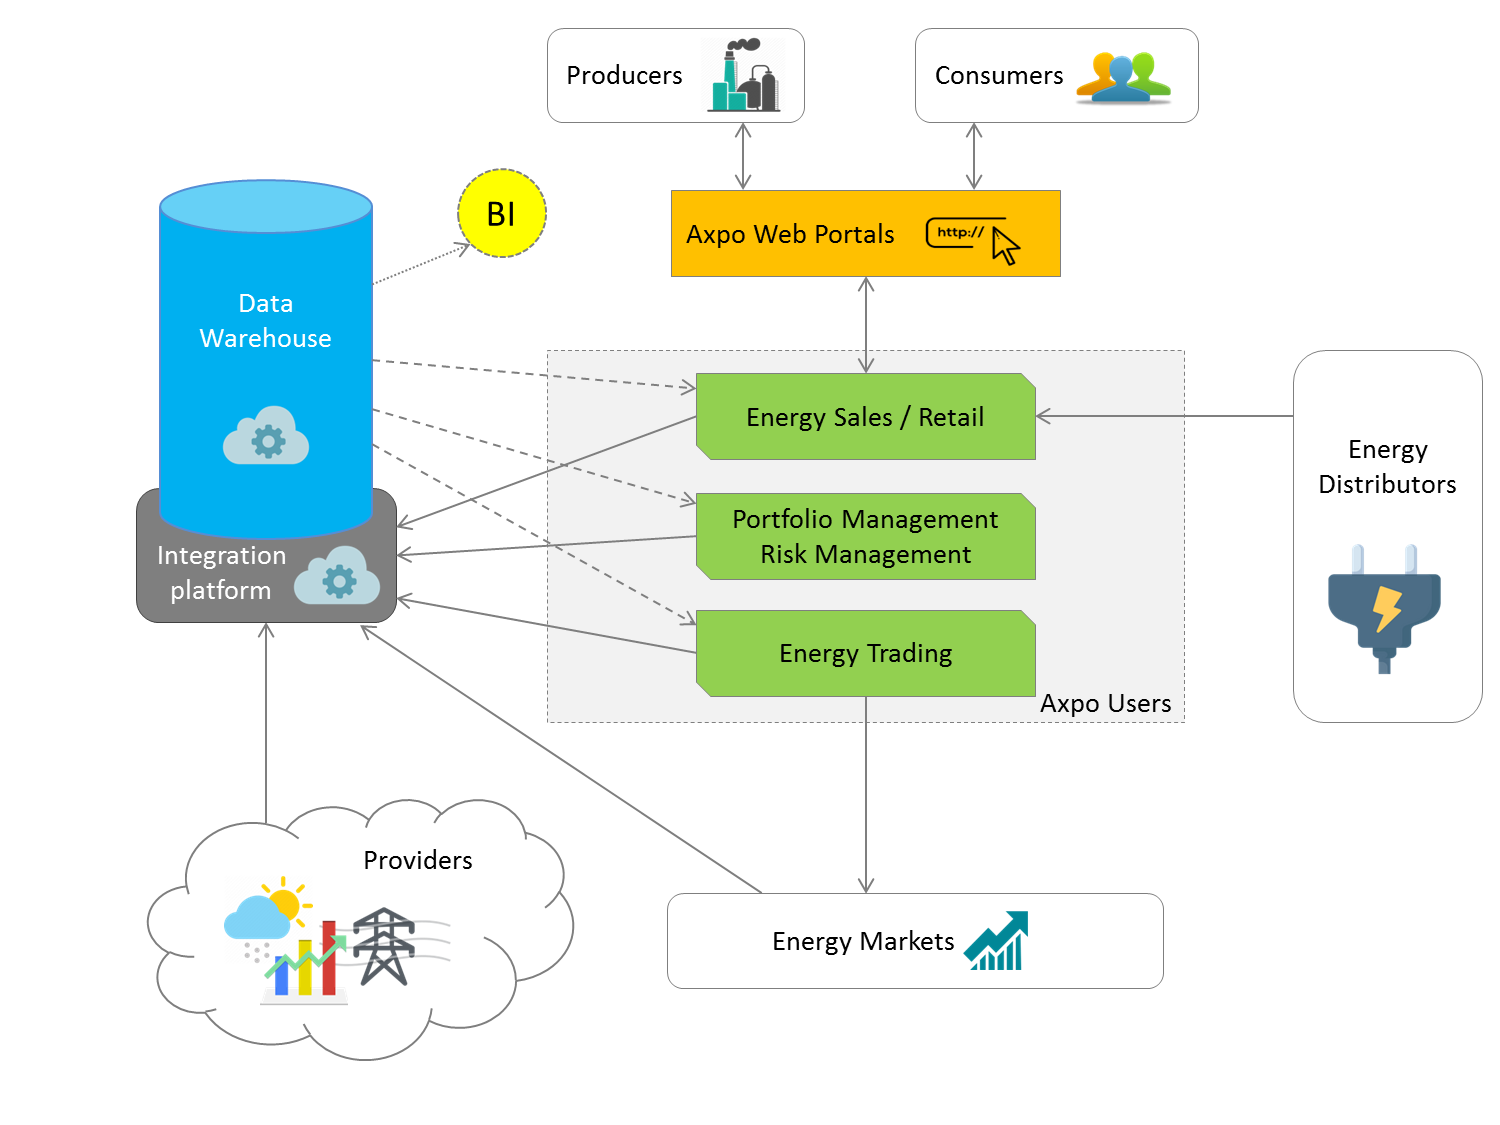
\includegraphics[width=\textwidth]{res/architecture/arch_end.png}
    \caption{Desired data communication structure among company departments and external data sources.}
    \label{fig:architecture:end}
\end{figure}

Figure \ref{fig:architecture:end} shows the desired outcome of the migration.

Each department is now expected to communicate only with the data warehouse and, in case information from different departments are needed, to extract these results from the data warehouse and not from the department itself.

This means that the data warehouse will always contain all the information and that they will always be up-to-date.

A similar situation applies also to data retrieve from external providers, which now will be retrieved by the cloud platform and not by specific users.

\paragraph{Business Intelligence}
    As we can see, Business Intelligence operations are much simpler compared to Figure \ref{fig:architecture:start}.
    
    In the old scenario, multiple sources need to be queried, and each source has its own integration layer.
    With the new architecture, all the data resides in one place, which means that analyses can be directly performed on the data warehouse.
    
    Moreover, the new architecture is expected to have higher performances, since operations can be executed on distributed and scalable machines.